\icode{N-MM-CA-L3-260625-001}
如图，光滑冰面上静止放置一表面光滑的斜面体，斜面体右侧一蹲在滑板上的小孩和其面前的冰块均静止于冰面上。某时刻小孩将冰块以相对冰面\,\qty{3}{m/s}的速度向斜面体推出，冰块平滑地滑上斜面体，在斜面体上上升的最大高度为\(h =\) \,\qty{0.3}{m}（\(h\)小于斜面体的高度）。已知小孩与滑板的总质量为\(m_1 =\) \,\qty{30}{kg}，冰块的质量为\(m_2 =\) \,\qty{10}{kg}小孩与滑板始终无相对运动。取重力加速度的大小\(g =\) \,\qty{10}{m/s^2}。
\begin{enumerate}[(1)]
    \item 求斜面体的质量;
    \item 通过计算判断,冰块与斜面体分离后能否追上小孩?
\end{enumerate}

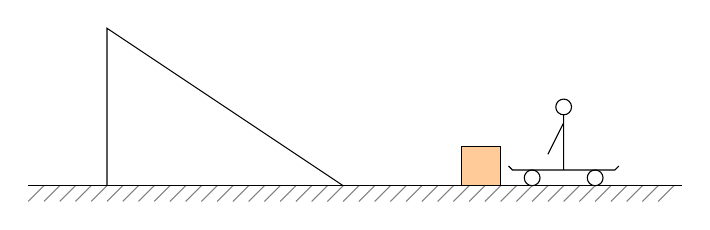
\begin{tikzpicture}
    \foreach \x in {-4,-3.8,...,4}
        \draw[gray] (\x,-.2)--++(.2,.2);
    \draw (-4,0)--(4.3,0);
    \draw (0,0)--(-3,2)--(-3,0);
    \draw[fill=orange!40] (1.5,0) rectangle(2,.5);
    \draw (2.4,.1) circle(.1) (3.2,.1)circle(.1) (2.8,1) circle(.1);
    \draw (2.1,.25)--(2.15,.2)--(3.45,.2)--(3.5,.25) (2.8,.9)--(2.8,.2) (2.8,.8)--(2.6,.4);
\end{tikzpicture}